\chapter{Hierarchical Representation}\label{chp:Hierarchical Representation}
% Authors: Hongyu (Florence) Lu, Michael Gold, Erica Dominic.
% Lecture date: 1.28.19

\section{The World as a Hierarchy}
% Authors: Hongyu (Florence) Lu, Michael Gold, Erica Dominic.
% Lecture date: 1.28.19

The world is inherently compositional and hierarchical: smaller pieces combine to form larger objects.
Humans interpret the world as a hierarchy; even the visual cortex in mammals is hierarchical in nature.

The goal of deep learning is to have a machine correctly extract hierarchical representations.
Ideally, a deep neural network should detect features at one level, then detect combinations of those features at the next level.
It is important to note that not every combination of features at one level exists in the next.

\subsection{Images}
% Authors: Hongyu (Florence) Lu, Michael Gold, Erica Dominic.
% Lecture date: 1.28.19

For example, from a patch of pixels, we want to detect edges (usually by an abrupt change in color of adjacent pixels).
From edges we can discern textons (e.g. corners, crosses).
From textons we can detect motifs, then parts of objects, and finally those parts can be pieced together to detect objects within the image.

Geometrically, if we take all $5\times5$ patches of pixels in an image, we will get a collection of $25$-dimensional vectors.
These vectors, however, would likely comprise a small (low-dimensional) part of $\mathbb{R}^{25}$.

\begin{figure}[ht]
\centering
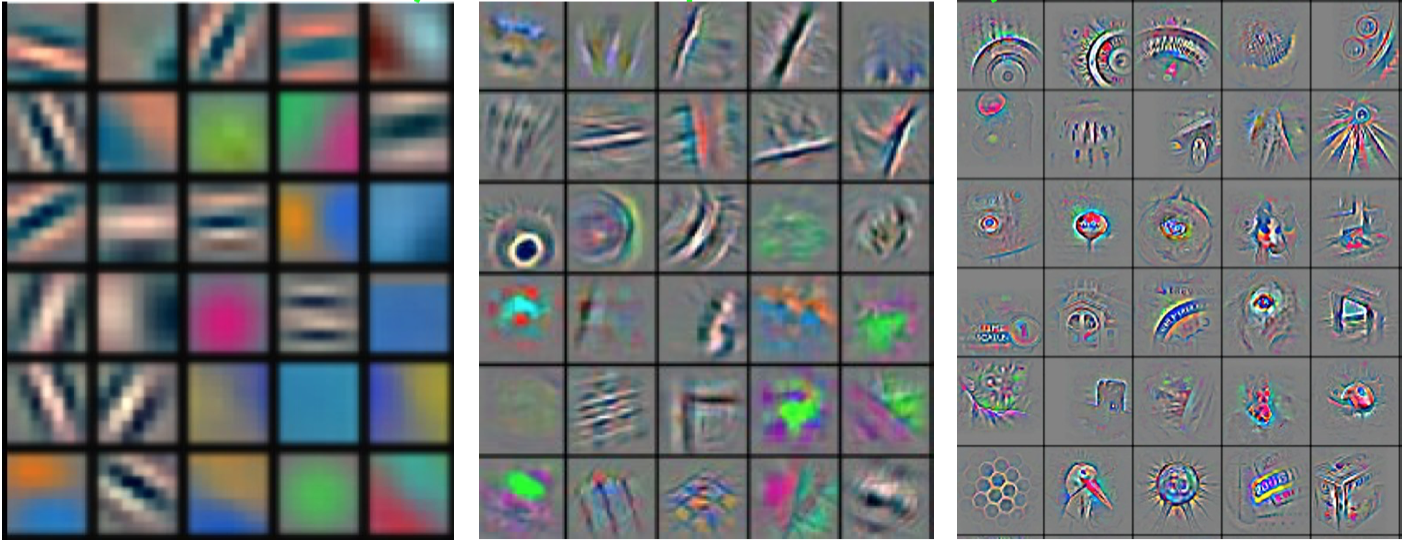
\includegraphics[width=100mm]{figs/cnn_hierarchy.png}
\caption{Hierarchy from a convolutional neural network}
\label{fig:cnn_hierarchy}
\end{figure}

\Cref{fig:cnn_hierarchy} shows an example from a convolutional neural network.
The left pane shows detected edges, color patches, and gradients.
The middle pane has pieced those attributes together to detect textures and shapes, such as round shapes and corners.
Finally, the right pane contains discernible parts of objects.

\subsection{Text}
% Authors: Hongyu (Florence) Lu, Michael Gold, Erica Dominic.
% Lecture date: 1.28.19

The same idea can be applied to textual analysis: combinations of characters become words, combinations of words make word groups, which assemble to make clauses, which can be grouped to make sentences, and finally a collection of sentences create a story.

Again, not every combination of features at one level becomes significant in the next, e.g. not every combination of words forms a valid sentence.

\subsection{Speech}
% Authors: Hongyu (Florence) Lu, Michael Gold, Erica Dominic.
% Lecture date: 1.28.19

An audio sample is just a single number, but the frequency content of a waveform can be represented by a feature vector, and those waveforms can be pieced together to form sounds, which can then be pieced together to form syllables, etc.
Ultimately phones and phonemes are formed and pieced into words.
